\begin{savequote}[6cm]
<< There's no need to go struttin' around and showin' off like that. 

\quad That's my job! >>
\qauthor{Rainbow Dash}
\end{savequote}

\chapter{Évaluation de performances}\label{chap:valid:perfs}
\chaptertoc

Afin d'effectuer l'observation de systèmes, nous avons présenté dans les chapitres précédent un SGFD extensible capable de se coupler avec un SGBD. Pour permettre le déploiement de cette solution sur tout type de plateforme, nous devons nous assurer que notre système n'est pas trop lourd en terme de performance. Dans ce chapitre, nous analysons les capacités de notre système pour choisir le meilleur plan de requête en fonction de la requête \textit{Astral} que nous lui soumettons.

Tout d'abord, en section~\ref{sec:valid:perfs:cadre}, nous présentons notre cadre expérimental. Ensuite, en section~\ref{sec:valid:perfs:flux}, nous nous intéressons à l'optimisation de la gestion de flux de données en soit avec le support du \textit{benchmark} reconnu \textit{Linear Road}. Nous traitons l'efficacité du couplage avec le SGBD dans la section~\ref{sec:valid:perfs:flux}. Enfin, nous concluons en section~\ref{sec:valid:perfs:conclusion}.

\section{Cadre d'expérimentation}\label{sec:valid:perfs:cadre}
Dans cette partie, nous présentons notre cadre expérimental. L'ensemble de la distribution Astronef-Asteroid est sous forme de \textit{bundles Java-OSGi}. Ainsi, ces prototypes peuvent être déployés sur toute plateforme possédant la technologie \textit{Java}. De plus, l'environnement \textit{OSGi} nous permet d'exploiter un environnement modulaire basé sur les architectures à service. La plateforme \textit{OSGi} doit embarquer le \textit{bundle} \textit{iPojo} (\url{http://felix.apache.org/site/apache-felix-ipojo.html}) pour pouvoir utiliser l'architecture à composants orientés service. Nous utilisons dans nos expériences la plateforme \textit{OSGi} \textit{Apache Felix} en version 3.0.2.

La distribution Astronef est fournie en 3 \textit{bundles} obligatoires à déployer pour pouvoir utiliser l'ensemble des fonctionnalités présentés dans cette thèse (api core parser). Ces \textit{bundles} embarquent aussi le moteur \textit{Prova} (\url{http://prova.ws}, version 3.1.9 minimale) capable d'exécuter l'ensemble des règles présentés. Les extensions à Astronef sont aussi sous forme de \textit{bundles} dont les classes dépendent de l'\textit{api}. C'est le cas du \textit{bundle} \textit{préférences} qui ajout les opérateurs \textbf{Best} et \textbf{KBest}. Astronef est disponible sous licence Apache 2.0 à l'adresse \url{http://astral.googlecode.com}.

Asteroid est une extension d'Astronef distribuée en un seul \textit{bundle}. Il embarque le SGBD \textit{H2} (\url{http://h2database.com}). Ce SGBD est entièrement en \textit{Java} ce qui permet une cohérence des technologies. Le binaire ou le code source d'Asteroid n'est actuellement pas disponible au public.

L'ordinateur utilisé pour les expérimentations utilise un processeur \textit{Intel Xeon}, quadri-cœur de fréquences 2.8Ghz. Il possède 6Go de mémoire vive et un disque dur d'une vitesse de 7200RPM. Le système d'exploitation utilisé est Linux Ubuntu 11.04. La plupart des expérimentations se sont faites dans un environnement clôt en isolant les processus sur trois cœurs dédiés afin d'éviter les interférences. Enfin, les expérimentations ont été faites dans des conditions les plus stables possibles, après que le \textit{JIT} soit passé, après initialisation des caches internes et avec un \textit{garbage collector} le plus stable possible.

Les performances sont mesurés par la latence d'un n-uplet. La latence est mesurée par la différence de timestamp système entre la source et le puit de la requête. Elle permet d'indiquer le temps total nécessaire au traitement d'un n-uplet. Le coût mémoire n'est pas compté, mais comme les trop grands coûts impactent le temps de traitement, notamment en \textit{Java} avec le \textit{GC}, nous supposons que cette métrique est représentative.

\section{Opérateurs de flux}\label{sec:contrib:astral:flux}
Astral repose sur deux concepts. Ainsi, il est nécessaire définir les opérateurs de flux vers relation (fenêtres) et de relation vers flux (streamers). Puis, nous définissons des opérateurs spécifiques : la gestion des modifications des relations temporelles et des \textit{batchs}.
\subsection{Fenêtres}
Comme nous l'avons vu dans la section~\ref{sec:rw:sgfd:modeles}, l'opérateur de fenêtre est un des opérateurs les plus étudiés dans la littérature. Toutefois, son comportement est encore flou sur certains points. La formalisation de son fonctionnement permet une meilleure spécification.
\subsubsection{Association position-\textit{batch}}
Avant de définir formellement l'opération de fenêtrage, nous avons besoin d'un outil pour gérer l'association entre la position d'un n-uplet et de son \textit{batch}. La fonction $\tau_S$ définit cette association (def~\ref{def:tau}). 
\begin{defi}[Fonction position-\textit{batch}]\label{def:tau}
    Soit $S$ un flux,

    La fonction $\tau_S : \N\to \TN$ est la fonction qui par une position (dans $\N$) donne l'identifiant du batch (dans $\TN$) du seul n-uplet ayant cette position.

    Par convention, $\tau_S(0)=(t_0,0)$.
\end{defi}

En corollaire de l'hypothèse des ordres~\ref{hyp:ordres}, la fonction $\tau_S$ est croissante non-stricte. Ainsi, il est possible de définir une pseudo inverse (cor~\ref{cor:rtau}) $\rtau_S$ capable de donner une position (la maximale) pour un \textit{batch} donné.
\begin{coro}[Fonction pseudo-inverse de $\tau$]\label{cor:rtau}
    Soit $S$ un flux,

    La pseudo-inverse $\rtau_S:\TN\to \N$ existe et correspond à la plus grande position du \textit{batch} donné en entrée. Si aucun \textit{batch} n'existe, le plus proche est utilisé. Formellement, $$\forall b \in \TN, \qquad \tau_S^{-1}(b) = \sum_{n=0}^{+\infty} n \indic_{[\tau_S(n),\tau_S(n+1)[}(b)$$
\end{coro}

\subsubsection{Description de séquences de fenêtres}
Afin de se rapprocher le plus possible d'un aspect déclaratif, il est nécessaire de décomposer l'opérateur de fenêtre en deux objets mathématiques : la description de son évolution et la séquence de fenêtres. Cette dernière prend une description en argument pour représenter la relation temporelle résultante. Le principe des descriptions de séquences de fenêtres tel que décrit dans la définition~\ref{def:dsf}) est assez simple puisqu'il suffit de décrire deux bornes ($\alpha$ et $\beta$) évoluant de manière discrète ainsi qu'un taux d'évaluation de ces bornes ($r$).

\begin{defi}[Description de Séquence de Fenêtre (DSF)]\label{def:dsf}
    Soient $\D$ et $\D'$ pouvant être $\T$ ou $\N$, une description de séquence de fenêtre (DSF) est un triplet $(\alpha,\beta,r)$ tel que :
\begin{itemize}
    \item $r \in \D$ est le taux d'évaluation des bornes de la fenêtre
    \item $\alpha$ et $\beta$ sont deux fonctions de $\N\to D'$ représentant l'évolution des bornes.
\end{itemize}

$\alpha(j)$ et $\beta(j)$ définissent les $j\eme$ valeurs des bornes. La première borne est donnée pour $j=0$. Ces fonctions se doivent de vérifier les propriétés suivantes (en considérant $\D=\D'=\T$) :
$$\forall j \in \N, \begin{cases} \alpha(j) \leq \beta(j) & \textrm{le début est avant la fin}\\ \alpha(j) \geq t_0 & \textrm{le début existe} \\ \beta(j) \leq jr + \beta(0) & \textrm{la fin est accessible} \end{cases}$$
    Les conditions pour les autres cas pour $\D$ et $\D'$ se déduisent par application des fonctions $\tau_S$ et $\rtau_S$.
\end{defi}

\begin{example}
    Nous souhaitons connaître tous les $100$ relevés de charge processeur, les $10$ derniers relevés. Dans ce cas, nous souhaitons obtenir une séquence de fenêtres positionnelles générées tous les $100$ n-uplets ($r=100\in \N$). Nous appliquons des bornes positionnelles $\alpha,\beta \in (\N\to\N)^2$. La première fenêtre contient du $91\eme$ n-uplet au $100\eme$. Ainsi : $\alpha(0) = 91$ et $\beta(0) = 100$. Sachant que l'évolution des bornes est linéaire, nous avons :
\begin{eqnarray*}
 \alpha(j) &=& 100j+91\\
 \beta(j) &=& 100j + 100\\
 r & = & 100
\end{eqnarray*}
\end{example}

La création de fenêtres nécessite d'associer les n-uplets du flux et le numéro de fenêtre décrit dans la \textit{DSF}. Pour cela, nous définissons en~\ref{def:gamma} une \textit{fonction d'attente} utilisant les identifiants de \textit{batchs}. Cette fonction donne le rang de la dernière fenêtre complète au moment du batch. Le terme \textit{attente} est lié au fait que l'évaluateur de fenêtre doit attendre le prochain changement de $\gamma$.
Nous retrouvons dans cette fonction le caractère \textit{bloquant} des fenêtres.
\begin{defi}[Fonction d'attente $\gamma$]\label{def:gamma}
    Soit $S$ un flux, soit $(\alpha,\beta,r)$ une DSF,

    La fonction d'attente de la DSF est une fonction $\TN \to \N$ permettant de trouver pour un identifiant de \textit{batch}, l'identifiant de la dernière fenêtre complétée.
\begin{itemize}
 \item  Si $r\in\T$, cette fonction est définie par $\gamma : (t,i) \mapsto \left\lfloor \frac{t-\beta(0)}{r} \right\rfloor$.
 \item  Si $r\in\N$, cette fonction est définie par $\gamma : (t,i) \mapsto \left\lfloor \frac{\rtau_S(t,i)-\beta(0)}{r} \right\rfloor$.
\end{itemize}
\end{defi}
\begin{example}
    En reprenant l'exemple précédent, après simplification nous obtenons : $$\gamma(b) = \left\lfloor \frac{\rtau_S(b)}{100}\right\rfloor-1.$$
    Si nous supposons que le flux produit un n-uplet par seconde (ainsi, $\rtau_S(t,i) = \lfloor t/1s \rfloor$) : alors $\gamma(1024s,0) = \left\lfloor \frac{1024}{100}\right\rfloor-1 = 9$. Nous avons bien la $10\eme$ fenêtre ($j=9$) comme la dernière fenêtre créée à l'instant 1024.
\end{example}

\subsubsection{L'opérateur}
Il devient désormais possible de définir un opérateur permettant de générer une relation temporelle à partir d'un flux donné. Cette relation temporelle change d'état avec l'instant défini par la fonction $\gamma$. De manière générale, une DSF peut être ramenée à une expression plus générale $(\alpha,\beta,\gamma)$ ce que nous utilisons pour la définition~\ref{def:fenetre} de séquence de fenêtres.
\begin{defi}[Opérateur de Séquence de Fenêtres]\label{def:fenetre}
	Soit $S$ un flux et $(\alpha, \beta, \gamma)$ une description de séquence,
	
	L'opérateur de séquence de fenêtres est défini par : $\forall b \in \TN$, 
	\begin{itemize}
		\item Si $\gamma(b) \geq 0$, 
		\begin{itemize}
			\item Si la description possède des bornes temporelles :
			$$S[\alpha,\beta,\gamma](b) = \left\{s\in S, \ (\alpha(\gamma(b)),0)\leq \BS(s) \leq (\beta(\gamma(b)),i)\right\}$$
			\item Si la description possède des bornes positions :
			$$E(b) = \left\{s\in S, \ \tau_S(\alpha(\gamma(b)))\leq \BS(s) \leq \tau_S(\beta(\gamma(b)))\right\}$$
			$$S[\alpha,\beta,\gamma](b) = \{s \in E(b) / (\#E(b) - \pos_{E(b)}(s)) \leq \beta(\gamma(b)) - \alpha(\gamma(b))$$
		\end{itemize}
		\item Si $\gamma(b) <0$ alors $S[\alpha,\beta,\gamma](b) = \emptyset$
	\end{itemize}
\end{defi}

Plusieurs remarques peuvent être formulées sur cette définition. Tout d'abord, les expressions sont différentes si les bornes sont positionnelles ou temporelles. Pour les fenêtres temporelles, l'opérateur inclut les n-uplets dont l'identifiant de \textit{batch} s'étend :
\begin{itemize}
	\item[\textbf{depuis}] le premier \textit{batch} de la fenêtre : $(\alpha(\gamma(t,i)),0)$, i.e. ceux dont le \textit{timestamp} est supérieur à la borne inférieure.
	\item[\textbf{jusqu'au}] dernier \textit{batch} de la fenêtre : $(\beta(\gamma(t,i)),i)$. Ce qui correspond au $i\eme$ \textit{batch} ayant le \textit{timestamp} inférieur ou égal à la borne.
\end{itemize}
Il est important de voir que $S[\alpha,\beta,\gamma]$ peut changer à l'arrivée d'un nouveau \textit{batch}, même si le \textit{timestamp} ne change pas. Ne pas inclure ces modifications ferait perdre des données à la fenêtre. Nous retrouvons les problématiques explorées dans la section~\ref{sec:rw:sgfd:modeles}.

Pour les fenêtres positionnelles, la gestion est plus délicate. Si nous considérons que le flux réparti ses \textit{batchs} (un n-uplet par \textit{batch}), alors $E(b) = S[\alpha,\beta,\gamma](b)$. Mais dans le cadre général, $E(b)$ contient l'ensemble des n-uplets potentiels et la séquence $S[\alpha,\beta,\gamma](b)$ en est un sous-ensemble dont la taille est exactement celle décrite dans la DSF (sélections des n-uplets les plus récents). De plus, nous remarquons que $\gamma$ en positionnel est défini en fonction de $\rtau_S$ qui fournit la position maximale en cas d'égalité de \textit{batchs}, ce qui nous garanti de couvrir l'ensemble des n-uplets concernés.


\begin{example}
	La figure~\ref{fig:contrib:astral:fenetres} montre l'évolution d'une séquence où la fenêtre glisse de $2$ secondes toutes les $2$ secondes ($r=2$) avec une taille constante de $3$ secondes. $t_0 = 0$ par simplicité ici. 
La première fenêtre possède les bornes $\alpha(0) = t_0+ 0s$ et $\beta(0) =t_0+3s$. Sachant que le glissement est de $2s$ la description de fenêtre est $$\forall j \in \N, \begin{cases} \alpha(j)  & =\ j*2s+t_0 \\ \beta(j) & = \ j*2s+3s+t_0\end{cases}$$
La relation temporelle générée par cette DSF peut être notée $S[2js,2js+3s,2s]$.  Le calcul de son état à un instant est simple. Prenons le \textit{batch} $(t_0+5.5s,0)$. La fenêtre à calculer est la fenêtre numérotée $\gamma(t_0+5.5s,0) = \left\lfloor \frac{t_0+5.5s-\beta(0)}{r}\right\rfloor = 1$. Ainsi : $S[2js,2js+3s,2s](t_0+5.5s,0) = F_1 = \{s_4,s_5,s_6,s_7,s_8\}$.
\end{example}
\begin{figure}[ht]
	\centering
	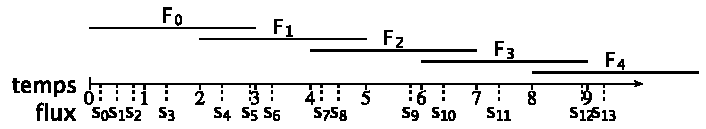
\includegraphics[width=0.7\textwidth]{contrib-astral-fenetres}
	\caption{Séquence de fenêtre de taille $3s$ glissante de $2s$}\label{fig:contrib:astral:fenetres}
\end{figure}

\begin{defi}[Exclusions de bornes de fenêtres]\label{def:exclufenetre}
    Soit $S$ un flux et $(\alpha,\beta,\gamma)$ une description de séquence de fenêtre,

    Les notations $S]\alpha,\beta,\gamma]$, $S[\alpha,\beta,\gamma[$ et $S]\alpha,\beta,\gamma[$ désignent les définitions de l'opérateur classique de séquence de fenêtre permettant d'exclure respectivement les bornes inférieures, supérieures ou les deux.
\end{defi}

\begin{example}
    En reprenant la définition de fenêtre sur 5 secondes : $(j*5s+t_0,j*5s+5s+t_0,5s)$. Nous remarquons que les fenêtres 0 et 1 contiennent les n-uplets dont le \textit{timestamp} est égal à $t_0+5s$. Ainsi, l'opérateur $S]jr+t_0,jr+r+t_0,r]$ avec $r=5s$ permet de retirer les n-uplets à ce \textit{timestamp} de cette fenêtre.
\end{example}

\subsubsection{Fenêtres partitionnées}
L'opérateur de fenêtres partitionnées est très utilisé pour appliquer la même séquence de fenêtres à des sous-flux. Les opérateurs partitionnés sont tous décrits de la même manière. Le principe, illustré dans la figure~\ref{fig:contrib:astral:partition} est de diviser le flux suivant un (ou des) attribut $A$ donné. Sur chacun de ces sous-flux est appliqué un opérateur quelconque. Le résultat est l'union des résultats de ces opérateurs.

\begin{figure}[ht]
	\centering
	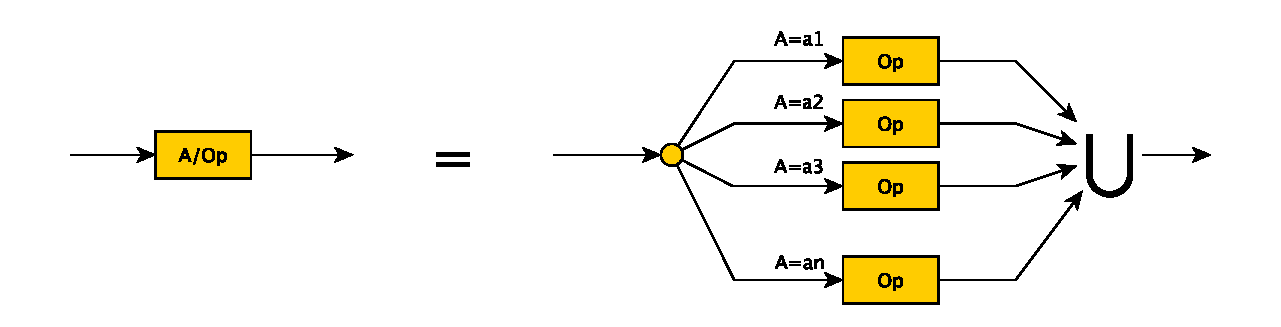
\includegraphics[width=0.9\textwidth]{contrib-astral-partition}
	\caption{Principe d'un opérateur partitionné}\label{fig:contrib:astral:partition}
\end{figure}

Ainsi, nous décrivons dans la définition~\ref{def:partition} de séquence de fenêtre partitionnée l'application de ces principes de partitionnement sur l'opérateur de séquence de fenêtre.
\begin{defi}[Séquence de fenêtre partitionnée]\label{def:partition}
	Soient $S$ un flux, $a_1,...,a_k$ un ensemble d'attributs du schéma de $S$, et $(\alpha,\beta,\gamma)$ une DSF,
	
	Soit $\cup^*$ l'union relationnelle conservant les identifiants physiques, 

	Alors, la séquence de fenêtres $(\alpha,\beta,\gamma)$ partitionnées par $a_1,...,a_k$ est définie par :
	$$S[a_1...a_k/\alpha,\beta,\gamma] = \mathop{\bigcup\null^*}_{a\in Dom(a_1,...,a_k)} (\sigma_{(a_1,...,a_k)=a} S)[\alpha,\beta,\gamma]$$
\end{defi}

Nous remarquons que nous utilisons la définition de l'union relationnelle conservant les identifiants physiques présentés dans la section précédente, ainsi l'ordre naturel décrit dans le flux d'entrée peut être retrouvé dans la relation de sortie.
\begin{example}
	L'exemple le plus courant est la représentation de l'état actuel d'un système à partir d'un flux. Supposons un flux d'entrée $CPU(appId,cpu,\t)$, nous donnant les relevés de charge de processeur. Soit la description de fenêtre rapportant le dernier n-uplet d'un flux : $(1j,1j,1)$. Nous pouvons obtenir la relation temporelle représentant pour chaque application $appId$, la dernière valeur connue de $cpu$ ainsi que le \textit{timestamp $\t$ de mesure} : $$CPU[appId/1j,1j,1]$$

	Cet exemple illustre comment nous pouvons passer d'un flux brut à une représentation (dynamique) d'un \textbf{contexte}. 
	
	La définition du partitionnement par l'union conservant les identifiants physiques permet d'avoir un ordre clair et intuitif sur la relation temporelle résultante. Lorsqu'un nouveau n-uplet entre dans cette relation (ou remplace l'ancien n-uplet), alors il est mis en bout. Avec l'union classique, il est nécessaire de définir l'ordre d'application des unions. Et les n-uplets auraient changé d'identifiants à chaque nouvel état de la fenêtre, ce qui est difficile à contrôler et à manipuler.
\end{example}

Par la suite, plusieurs notations simplifiées sont utilisées pour désigner des descriptions de fenêtres courantes décrites dans le tableau~\ref{tab:windows}.
\begin{table}[ht]
\centering
\begin{tabular}{c||p{0.4\textwidth}|p{0.4\textwidth}}
  & Définition & Équivalence \\ \bottomrule
 $[L]$ & $[j,j,1]$ &  \\ 
 & \multicolumn{2}{p{0.8\textwidth}}{La séquence de fenêtre où chaque fenêtre ne contient que le dernier n-uplet du flux. Cette séquence est égale à $[B]$ si le flux répartit ses n-uplets avec un n-uplet par \textit{batch}.} \\ \hline
 $[B]$ & $]\tau_S^{-1}(\tau_S(j)^-),j,1]$ & $\{s\in S, \BS(s) = \tau_S\circ\tau_S^{-1}(b)\}$ \\ 
 & \multicolumn{2}{p{0.8\textwidth}}{Séquence de fenêtre où chaque fenêtre contient le dernier \textit{batch}.} \\\hline
 $[\infty]$ & $[0,j,1]$ & $\{s\in S, \BS(s) \leq b\}$ \\
 & \multicolumn{2}{p{0.8\textwidth}}{Séquence cumulative contenant tout le flux jusqu'au \textit{batch} courant.} \\\hline
 $[T\ r\ s]$ & $]\max(sj-r+t_0,t_0),sj+t_0,s]$ &  \\
 & \multicolumn{2}{p{0.8\textwidth}}{Fenêtre temporelle de taille $r$ se déplaçant toutes les $s$ unités de temps.} \\\hline
 $[P\ r\ s]$ & $]\max(sj-r,0),sj,r]$ &  \\
 & \multicolumn{2}{p{0.8\textwidth}}{Fenêtre positionnelle de taille $r$ n-uplets se déplaçant tous les $s$ n-uplets.} \\
 \toprule
\end{tabular}
\caption{Liste des fenêtres courantes} \label{tab:windows}
\end{table}
Il est important de noter que les équivalences citées sont non triviales, des démonstrations formelles sont fournies en annexes~\ref{misc:fenetres}.

\subsection{Streamers}
La classe des \textit{streamers} est l'ensemble des opérateurs produisant un flux à partir d'une relation. Son utilisation, après l'application d'une fenêtre, permet la création d'un flux résultant. La définition des streamers est découpée en deux parties, d'abord la définition de la réécriture de \textit{timestamp} qui permet d'ajouter le \textit{timestamp} aux données produites, et ensuite la définition de l'opérateur.
\subsubsection{Réécriture de \textit{timestamp}}
Il est nécessaire de gérer les identifiants physiques. En effet, si un n-uplet est envoyé plusieurs fois dans le flux résultat, il y a conflit si $\varphi$ n'est pas modifié. De plus, tout flux doit avoir un attribut $\t$. Cet attribut doit être créé ou remplacé pour assurer l'hypothèse des ordres. Le principe est que le n-uplet $s\in R(b)$ doit être envoyé dans le flux au \textit{batch} $(t_s,i_s)$, alors nous devons envoyer le n-uplet $\Psi_b(s,t_s)$ décrit dans la définition~\ref{def:stamping}.
\begin{defi}[Fonction de réécriture de \textit{timestamp}]\label{def:stamping}
    Soit $R$ une relation de schéma $A$, $b$ un batch,

    Soit $\I^S = \TN\times \I_R$ le $\Phi$-espace ordonné de manière naturelle,

    La fonction de réécriture de \textit{timestamp} appliquée à $R(b)$ est définie par : 
$$\forall s\in R(b), \ \forall t_s\in\T, \ \Psi_b(s,t_s) = \{(\t,t_s), (\varphi, (b,s(\varphi)))\}\bigcup_{a\in A\backslash\{\varphi,\t\}}\{(a,s(a))\}$$
\end{defi}

Cette définition assure que les nouveaux n-uplets du flux vérifient les propriétés suivantes : 
\begin{itemize}
 \item Ils ont pour \textit{timestamp} $t_s$ le moment où il a été estampillé.
 \item Ils ont un identifiant physique (et du coup une position) plus grand que les identifiants précédents.
 \item L'ordre positionnel de $R(b)$ est préservé.
\end{itemize}
Nous pouvons définir des \textit{streamers} dit sensibles dans la définition~\ref{def:streamers}). Ces \textit{streamers} réagissent aux changements de $R$ et produisent un flux en conséquence.
\begin{defi}[\textit{Streamers} sensibles]\label{def:streamers}
    Soit $R$ une relation,

    Les \textit{streamers} sensibles sont les opérateurs créateurs d'un flux $S$ défini à partir des changements de $R$, trois types sont définis :
\begin{itemize}
 \item Le \textit{streamer} d'insertion, envoyant les nouveaux n-uplets : $\IS(R)$, $$s\in R(t,i) \wedge s\not\in R((t,i)^-) \equ s'=\Psi_{(t,i)}(s,t)\in S \wedge \BS(s') = (t,i)$$
 \item Le \textit{streamer} de suppression, envoyant les n-uplets disparus : $\DS(R)$, $$s\not\in R(t,i) \wedge s\in R((t,i)^-) \equ s'=\Psi_{(t,i)^-}(s,t)\in S \wedge \BS(s') = (t,i)$$
 \item Le \textit{streamer} d'envoi, envoyant tous les n-uplets présents : $\RSu(R)$, $$s\in R(t,i) \neq R((t,i)^-) \equ s'=\Psi_{(t,i)}(s,t)\in S \wedge \BS(s') = (t,i)$$
\end{itemize}
\end{defi}

Nous avons constitué la chaîne complète permettant de traiter les flux de données : flux vers relation, relation vers relation, et relation vers flux. Nous allons explorer un exemple complet pour montrer la clarté d'expression issue de l'algèbre.

\begin{example}
    Le flux d'alerte avec pour attributs (deviceId, avgcpu, $\t$) représente que l'équipement \textbf{deviceId} au \textit{timestamp} $\t$ a eu une charge moyenne \textit{avgcpu} supérieure à 25\%. La moyenne est calculée sur 5 min toutes les minutes.

    Pour former ce flux, il est nécessaire de joindre le flux \textbf{CPU} avec \textbf{Applications} afin de pouvoir associer le bon \textit{deviceId} à l'\textit{appId}. Or, cette opération est interdite à moins de faire une fenêtre sur le flux. Nous pourrions utiliser une fenêtre telle que le dernier \textit{batch} $[B]$, mais comme il est nécessaire d'obtenir une fenêtre temporelle pour le calcul de moyenne, nous pouvons appliquer la description appropriée : $$CPU[T\ 5min\ 1min]\Join Applications.$$

    Appliquons l'opération d'agrégation sur cette relation pour obtenir la moyenne. Puis nous pouvons sélectionner les n-uplets la moyenne est supérieure à 25\%. Enfin, le flux doit être créé à partir de la relation temporelle représentant les équipements supérieurs à 25\% de charge pendant les 5 dernières minutes. Ici une ambiguïté réside dans l'énoncé. Souhaitons-nous avoir le flux des nouveaux équipements ayant ce problème ou souhaitons-nous être notifiés à chaque vérification ? Ce critère va influencer le choix du \textit{streamer} : $\IS$ ou $\RSu$. Prenons le premier, nous obtenons la requête suivante : 
    $$\IS\left(\sigma_{avgcpu \geq 25} \ \null_{deviceId}\G_{avg_{cpu}^{avgcpu}} (CPU[T\ 5min\ 1min]\Join Applications)\right)$$
\end{example}

D'autres streamers peuvent être construits pour effectuer l'insertion de données dans le flux résultat de manière périodique comme le présente la définition~\ref{def:rsr}.
\begin{defi}[\textit{Streamers} périodiques]\label{def:rsr}
    Soit $R$ une relation,

    Les \textit{streamers} périodiques sont les opérateurs créateurs d'un flux $S$ où les insertions ont lieu périodiquement. Le \textit{streamer} $\RS{r}$ est défini par un taux temporel $r$ et la propriété :
$$s\in R(t,i) \wedge t-t_0\equiv 0[r]\equ s'=\Psi_{(t,i)}(s,t)\in S \wedge \BS(s') = (t,i)$$
\end{defi}

Nous avons maintenant défini des opérateurs permettant de couvrir la plupart des opérations. Toutefois, deux opérateurs sont encore à définir pour certaines opérations plus particulière.
\subsection{Manipulation temporelle}\label{sec:contrib:astral:manipulation}
Contrairement à l'algèbre relationnelle, les relations sont temporelles ici. Elles changent au cours de l'exécution de la requête. Il n'existe pas d'opérateurs capables de contrôler ces changements. L'opérateur de manipulation temporelle permet de sélectionner, pour l'instant présent, un état passé d'une relation. Tout d'abord, définissons une transformation temporelle avec la définition~\ref{def:transformation} permettant de sélectionner l'instant voulu sur la relation temporelle. La seule contrainte de cette transformation est l'impossibilité de regarder dans le futur. Nous pouvons ainsi définir l'opérateur de manipulation temporelle (def~\ref{def:manipulation}) qui applique cette transformation à la relation temporelle.
\begin{defi}[Transformation temporelle]\label{def:transformation}
    Une transformation temporelle est une fonction de $\TN\to\TN$ telle que $\forall b\in\TN, f(b) \leq b$.
\end{defi}

\begin{defi}[Opérateur de manipulation temporelle]\label{def:manipulation}
    Soient $R$ une relation, $c$ une condition sur $\TN$ et $f$ une transformation temporelle,

    Alors l'opérateur de manipulation temporelle est défini par $$\D_c^f(R) = b \mapsto \begin{cases} R(f(b)) & \textrm{ si } c(b) \\ \emptyset & \textrm{ sinon}\end{cases}$$
\end{defi}

Plusieurs fonctions classiques ont une utilité directe :
\begin{itemize}
 \item $\mathrm{freeze}^{t_s}(t,i)=(t_s,0)$ si $t \geq t_s$. Permet de figer une relation temporelle à un instant précis, plus aucun changement n'est retransmis à partir de ce point. La relation résultante de cette opération est notée $R^{t_s}$. Un cas particulier est lorsque $t_s=t_0$. Dans ce cas la relation n'a qu'un seul état. Grâce à cette opération, nous sommes capables de faire une \textbf{interrogation instantanée} sur des relations temporelles.
 \item $\mathrm{period}^r(t,i)=\left(\left\lfloor\frac{t-t_0}{r}\right\rfloor r + t_0, 0\right)$ met à jour la relation de manière périodique avec un taux de rafraîchissement $r$.
 \item $\mathrm{change}_S(t,i)=\tau_S\circ\rtau_S$ met à jour la relation à chaque fois qu'un \textit{batch} est inséré dans $S$. Le même principe permet une mise à jour \textit{à chaque fois que la relation $R'$ change}.
\end{itemize}

Cette dernière fonction a un impact particulier lors de la jointure de deux relations temporelles. Dans la jointure (ou au sens large le produit cartésien) telle que nous l'avons définie, si un changement est appliqué d'un côté ou de l'autre, un nouveau calcul de jointure est effectué. Ce comportement peut ne pas être souhaité dans la pratique où nous pourrions souhaiter que seule une branche soit déclencheur de calcul et l'autre soit passive. La jointure semi-sensible permet cette opération. Dans la définition~\ref{def:ssjoin} le résultat $R_1 \ssjoin R_2$ n'est pas mis à jour au changement de $R_2$ mais au changement de $R_1$ avec l'état de $R_2$ correspondant.

\begin{defi}[Jointure semi-sensible]\label{def:ssjoin}
    Soient $R_1$ et $R_2$ deux relations temporelles,

    Soit $\mathrm{change}_{R_1}$ la transformation temporelle telle que $\mathrm{change}_{R_1}(b)$ correspond au dernier changement de $R_1$ inférieur ou égal à $b$,

    La jointure semi-sensible est définie par :
        $$R_1\ssjoin R_2 = R_1 \Join \D^{\mathrm{change}_{R_1}}(R_2)$$
\end{defi}
\begin{example}
    $$DeviceCPU=\IS(\Pi_{deviceId,deviceName,cpu}(CPU[B]\Join Applications)\ssjoin Devices)$$

Le flux résultat $DeviceCPU$ correspond au flux \textit{CPU} originel sur lequel nous avons remplacé l'attribut \textit{appId} par les attributs \textit{deviceId} et \textit{deviceName} qui sont plus intéressants d'un point de vue de l'observation. Si \textit{Devices} est mise à jour (pour changer son statut) en utilisant la jointure simple, la relation temporelle change d'état. Ce qui provoque l'envoi d'un nouveau n-uplet dans le flux. L'opérateur de jointure semi-sensible empêche ce cas puisque les mises à jour sont cadencées par celles de $CPU[B]\Join Applications$ c'est-à-dire $CPU[B]$ soit encore les \textit{batchs} de $CPU$ et non la relation \textit{Devices}.
\end{example}

\subsection{Spread}
Enfin, le dernier opérateur est celui évoqué lors de la conception des \textit{batchs} dans~\cite{Jain:spread}. Il est nécessaire d'avoir un opérateur pour manipuler les \textit{batchs} afin de modifier la fonction $\BS$ d'un flux sans toucher à ses données.

L'opérateur de réinitialisation des \textit{batchs} (def~\ref{def:spreadall}, \textit{spread all} dans la littérature) permet de rassembler les \textit{batchs} multiples pour chaque \textit{timestamp} en un seul. Ceci permet de réorganiser le flux.
\begin{defi}[Réinitialisation des batch]\label{def:spreadall}
Soit $S$ un flux,

Le flux $S$ réinitialisé noté $\lhd S$ vérifie :
$$\forall s\in S, \textrm{ alors } s \in \lhd S, \textrm{ et }\B{\lhd S}(s) = (s(\tau),0)$$
\end{defi}

L'opérateur \textit{spread} décrit dans la définition~\ref{def:spread} permet de découper les \textit{batchs} présents dans un flux en plusieurs nouveaux. Le découpage se fait sur l'ordre induit par ses attributs. Ceci permet par exemple de partitionner selon un identifiant.
\begin{defi}[\textit{Spread}]\label{def:spread}
Soient $S$ un flux de schéma $A$, et $a$ un attribut de $S$,

Soit $\I^S = \TN\times \I_R$ le $\Phi$-espace ordonné de manière lexicographique,

Alors le flux $S$ raffiné par l'attribut $a$ noté $\rhd_{a} S$ vérifie :
$\forall s_1, s_2\in S^2, \textrm{ alors } s_1', s_2' \in (\rhd_a S)^2,$ tel que :
\begin{eqnarray*}
b_1=\B{\rhd_a S}(s_1') < b_2=\B{\rhd_a S}(s_2') &\equ & \BS (s_1) < \BS (s_2)\\ & & \quad \vee \ \left(\BS (s_1) = \BS (s_2)\right. \\ & & \quad\quad \quad\quad\wedge \ \left.s_1(a) < s_2(a)\right)
\end{eqnarray*}

Ainsi que $s_i' = \{(\varphi, (b_i,s_i(\varphi)))\}\bigcup_{x\in A\backslash\{\varphi\}}\{(x,s(x))\}$, pour $i\in\{1,2\}$
\end{defi}

Originellement, si pour l'opérateur \textit{spread}, aucun attribut n'est mentionné, alors tous les n-uplets sont étalés dans des batchs séparés de manière non déterministe. Dans notre algèbre, l'attribut $\varphi$ et l'ordre positionnel permettent de définir l'ordre des \textit{batchs} comme l'ordre positionnel : $\rhd = \rhd_\varphi$. À l'inverse, en appliquant $\lhd$, nous définissons l'ordre des \textit{batchs} comme l'ordre temporel.

\begin{example}
Sachant le contenu du flux \textbf{CPU}(appId, value, $\t$) :

\begin{center}\noindent\begin{tabular}{|c|c|c|} \bottomrule
(1,0) & (1,1) & (2,0) \\ \hline
\begin{tabular}{c}
$(1,20,1)$ \\
$(1,25,1)$ \\
$(2,22,1)$ \\
\end{tabular} &
\begin{tabular}{c}
$(4,10,1)$ \\
$(1,25,1)$ \\
$(4,12,1)$ \\
\end{tabular} &
\begin{tabular}{c}
$(2,23,1)$ \\
$(6,64,1)$ \\
\end{tabular} \\ \toprule
\end{tabular}
\end{center}

 $\lhd\ CPU$ : L'application de l'opérateur de réinitialisation des \textit{batchs} regroupe tous les n-uplets simultanés dans le même \textit{batch}.
 
\begin{center}\noindent\begin{tabular}{|c|c|} \bottomrule
(1,0) & (2,0) \\ \hline
\begin{tabular}{c}
$(1,20,1)$ \\
$(1,25,1)$ \\
$(2,22,1)$ \\
$(4,10,1)$ \\
$(1,25,1)$ \\
$(4,12,1)$ \\
\end{tabular} &
\begin{tabular}{c}
$(2,23,1)$ \\
$(6,64,1)$ \\
\end{tabular} \\ \toprule
\end{tabular}
\end{center}

 $\rhd_{appId}\ CPU$ : L'utilisation du \textit{spread} sur l'identifiant permet d'affiner les \textit{batchs} originels en garantissant que chaque \textit{batch} ne contienne qu'une valeur de \textit{appId}.
 
\begin{center}\noindent\begin{tabular}{|c|c|c|c|c|c|} \bottomrule
(1,0) & (1,1) & (1,2) & (1,3) & (2,0) & (2,1) \\ \hline
\begin{tabular}{c}
$(1,20,1)$ \\
$(1,25,1)$ \\
\end{tabular} &
\begin{tabular}{c}
$(2,22,1)$ \\
\end{tabular} &
\begin{tabular}{c}
$(1,25,1)$ \\
\end{tabular} &
\begin{tabular}{c}
$(4,10,1)$ \\
$(4,12,1)$ \\
\end{tabular} &
\begin{tabular}{c}
$(2,23,1)$ \\
\end{tabular} &
\begin{tabular}{c}
$(6,64,1)$ \\
\end{tabular} \\ \toprule
\end{tabular}
\end{center}

$\lhd\rhd_{appId}\ CPU$ : La combinaison de la réinitialisation et du \textit{spread} permettent d'avoir un \textit{batch} par \textit{timestamp} affecté à une valeur d'\textit{appId}.

\begin{center}\noindent\begin{tabular}{|c|c|c|c|c|} \bottomrule
(1,0) & (1,1) & (1,2) & (2,0) & (2,1) \\ \hline
\begin{tabular}{c}
$(1,20,1)$ \\
$(1,25,1)$ \\
$(1,25,1)$ \\
\end{tabular} &
\begin{tabular}{c}
$(2,22,1)$ \\
\end{tabular} &
\begin{tabular}{c}
$(4,10,1)$ \\
$(4,12,1)$ \\
\end{tabular} &
\begin{tabular}{c}
$(2,23,1)$ \\
\end{tabular} &
\begin{tabular}{c}
$(6,64,1)$ \\
\end{tabular} \\ \toprule
\end{tabular}
\end{center}
\end{example}

Nous avons maintenant présenté l'ensemble des opérateurs de l'algèbre Astral. Nous sommes désormais capables d'exprimer une requête continue (et instantané avec l'aide de la manipulation temporelle) avec une grande clarté et sans ambiguïté sémantique. Nous allons maintenant, définir l'équivalence de requête avec des \textit{timestamps} de départs $t_0$ différents.
\section{Choix du plan de jointure dans Asteroid}\label{sec:valid:perfs:couplage}
En section~\ref{sec:contrib:asteroid:reecriture:join}, nous avons présenté un opérateur capable de faire une jointure $\ssjoin$ entre une relation temporelle d'Astronef et une relation issue d'un SGBD. Deux plans ont été présenté : le plan \textbf{P1} applique la jointure dans Astronef en utilisant la relation temporelle issue du SGBD comme cache local ; le plan \textit{P2} quant à lui exécute l'opération de jointure à l'intérieur du SGBD pour exploiter ses capacités. Alors que l'optimisation poussant les opérateurs au plus proche du SGBD semble efficace dans la plupart des cas, nous voyons dans cette section que ce n'est pas toujours le cas pour cette opération.

\subsection{Jointure sur une relation statique}
Nous exécutons ici la requête $CPUMem$ présenté en section~\ref{sec:valid:domvision:requetes:historisation}. Pour rappel, cette requête implique une jointure avec $Application \Join Monitorable$ pour pouvoir identifier le flux de métriques processeurs et mémoires. Voici les paramètres d'expérimentations que nous fixons :
\begin{itemize}
	\item Les relations temporelles \textit{Monitorable} et \textit{Applications} sont considérées statiques
	\item La cardinalité d'\textit{Applications} est $N$
	\item La cardinalité de \textit{Devices} est $0.2N$ et celle de \textit{Monitorable} est de $1.2N$
	\item Il existe un index \textit{Application(monitorableId)}, \textit{Monitorable(monitorableId)} et sur \textit{Monitorable(name)}
	\item Il y a toujours suffisamment de mémoire pour exécuter les requêtes \textit{SQL}.
\end{itemize}

La requête \textit{SQL} automatiquement généré et donnée aux composants \textit{dbjoin} et \textit{dbsource} est la suivante :
\begin{lstlisting}[language=SQL]
SELECT deviceId as monitorableId, name 
FROM Application NATURAL JOIN Monitorable
\end{lstlisting}

\begin{figure}[ht]
	\centering
	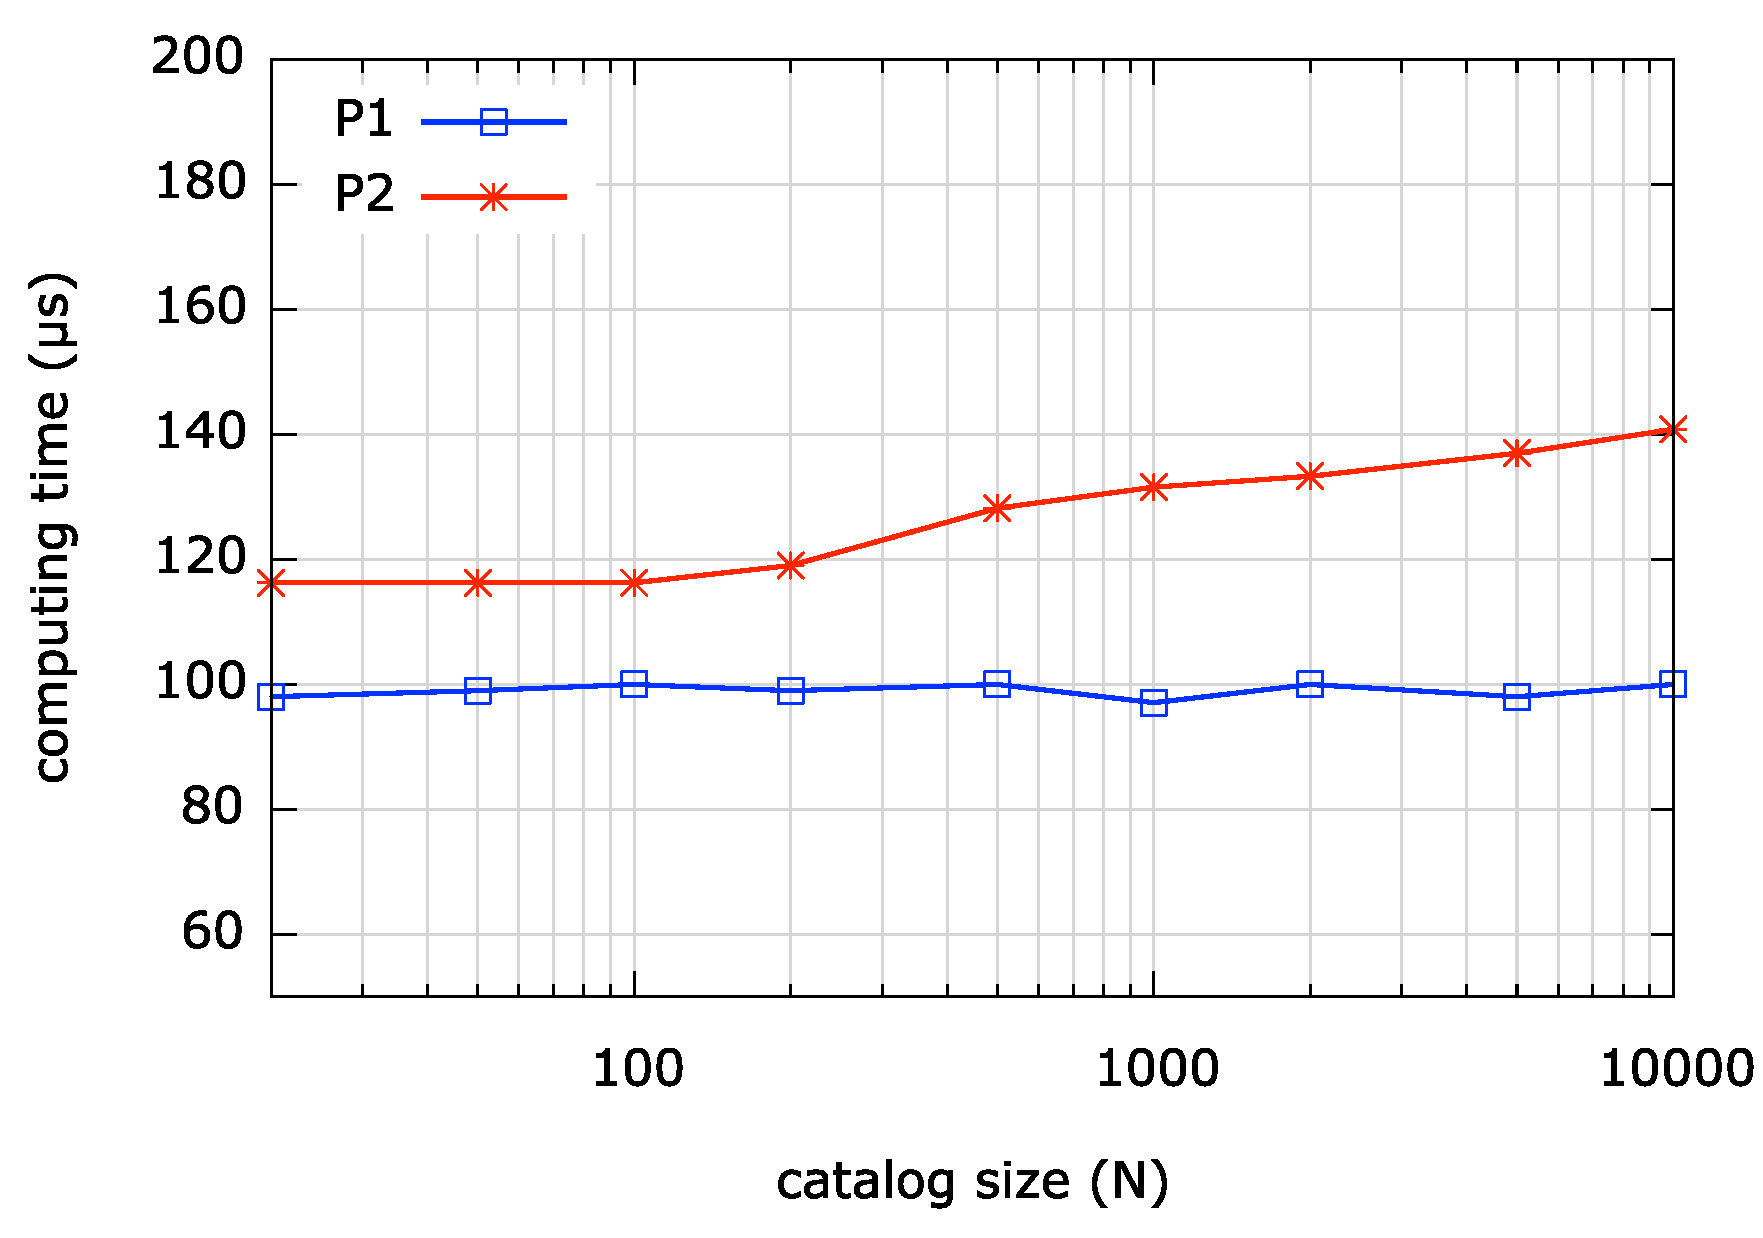
\includegraphics[width=0.66\textwidth]{valid-perfs-asteroid-static}
	\caption{Performance d'une jointure sur catalogue statique}\label{fig:valid:perfs:asteroid:static}
\end{figure}

\textbf{Résultats} : La figure~\ref{fig:valid:perfs:asteroid:static} montre la latence des deux plans de requête \textbf{P1} et \textbf{P2}. Les expérimentations ont montré que le plan \textit{P1} est meilleur et plus stable sur $N$. Bien entendu, cela ne pourra pas être le cas pour des valeurs très larges de $N$. Dans notre cadre expérimental, le \textit{hash-join} ne semble pas être le facteur limitant à $100\mu s$, car cela consiste à interroger une table de hachage constituée une seule fois. Le coût du \textit{scheduling} et d'autres tâches de l'intergiciel deviennent des facteurs limitants. 

Le plan \textbf{P2} est plus coûteux car pour chaque n-uplet, le composant doit se connecter au SGBD et exécuter la requête. Bien que la requête soit préparé, cela introduit un coût supplémentaire. Ce plan utilise l'index stocké sur disque dur, mais ses performances sont moindre comparé à un accès direct à une table de hachage en mémoire.

Si les relations \textit{Monitorable} ou \textit{Applications} sont mis à jour, cela introduit un surcout pour recalculer la table de hachage. Toutefois, le coût est absorbé au fur et à mesure du temps si les relations sont mises à jour rarement. Ainsi, le choix de \textbf{P1} est le meilleur pour la jointure avec des relations stables.

\subsection{Jointure sur un agrégat historique}
Dans cette seconde expérimentation, nous exécutons la requête $HistAvgCPU$ vu dans la section~\ref{sec:valid:domvision:requetes:alerte}. Pour rappel, cette requête joint une relation temporelle avec un agrégat effectué sur historique. Voici les paramètres de notre expérience :
\begin{itemize}
	\item L'historique est mise à jour dès que possible par un processus de collecte extérieur ($CPUMem$ par exemple).
	\item Il existe $D$ identifiants d'équipement et $M$ valeurs historique par identifiants.
	\item Il y a un index sur \textit{HistCPU(monitorableId)}.
\end{itemize}

La requête \textit{SQL} générée et donnée en paramètre à \textit{dbjoin} et \textit{dbsource} est la suivante : 
\begin{lstlisting}
SELECT monitorableId, AVG(cpu) as avg FROM HistCPU GROUP BY monitorableId
\end{lstlisting}

\begin{figure}[ht]
\subfigure[Performance globale]{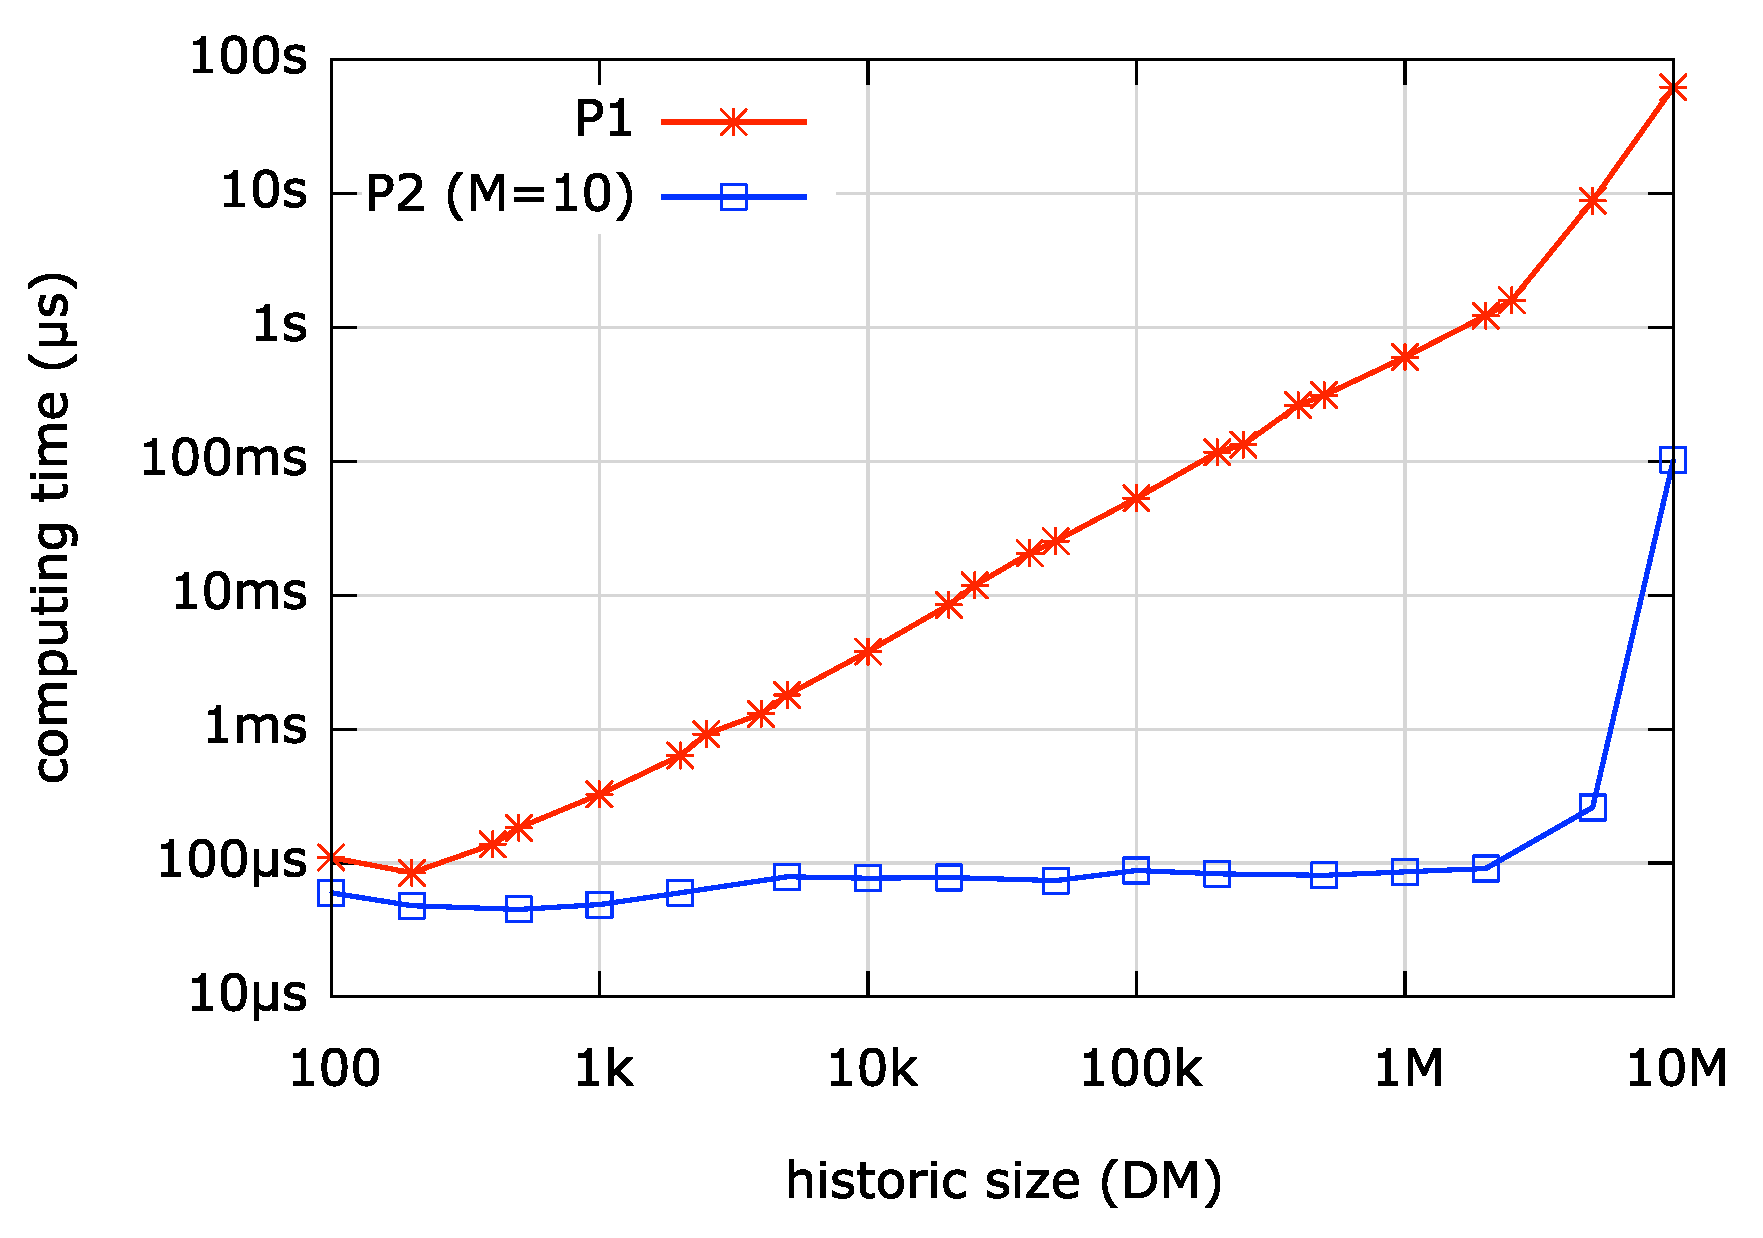
\includegraphics[width=0.48\linewidth]{valid-perfs-asteroid-aggregate}\label{fig:valid:perfs:asteroid:aggregate}}
\subfigure[Performance de l'agrégat avec sélection sur identifiant]{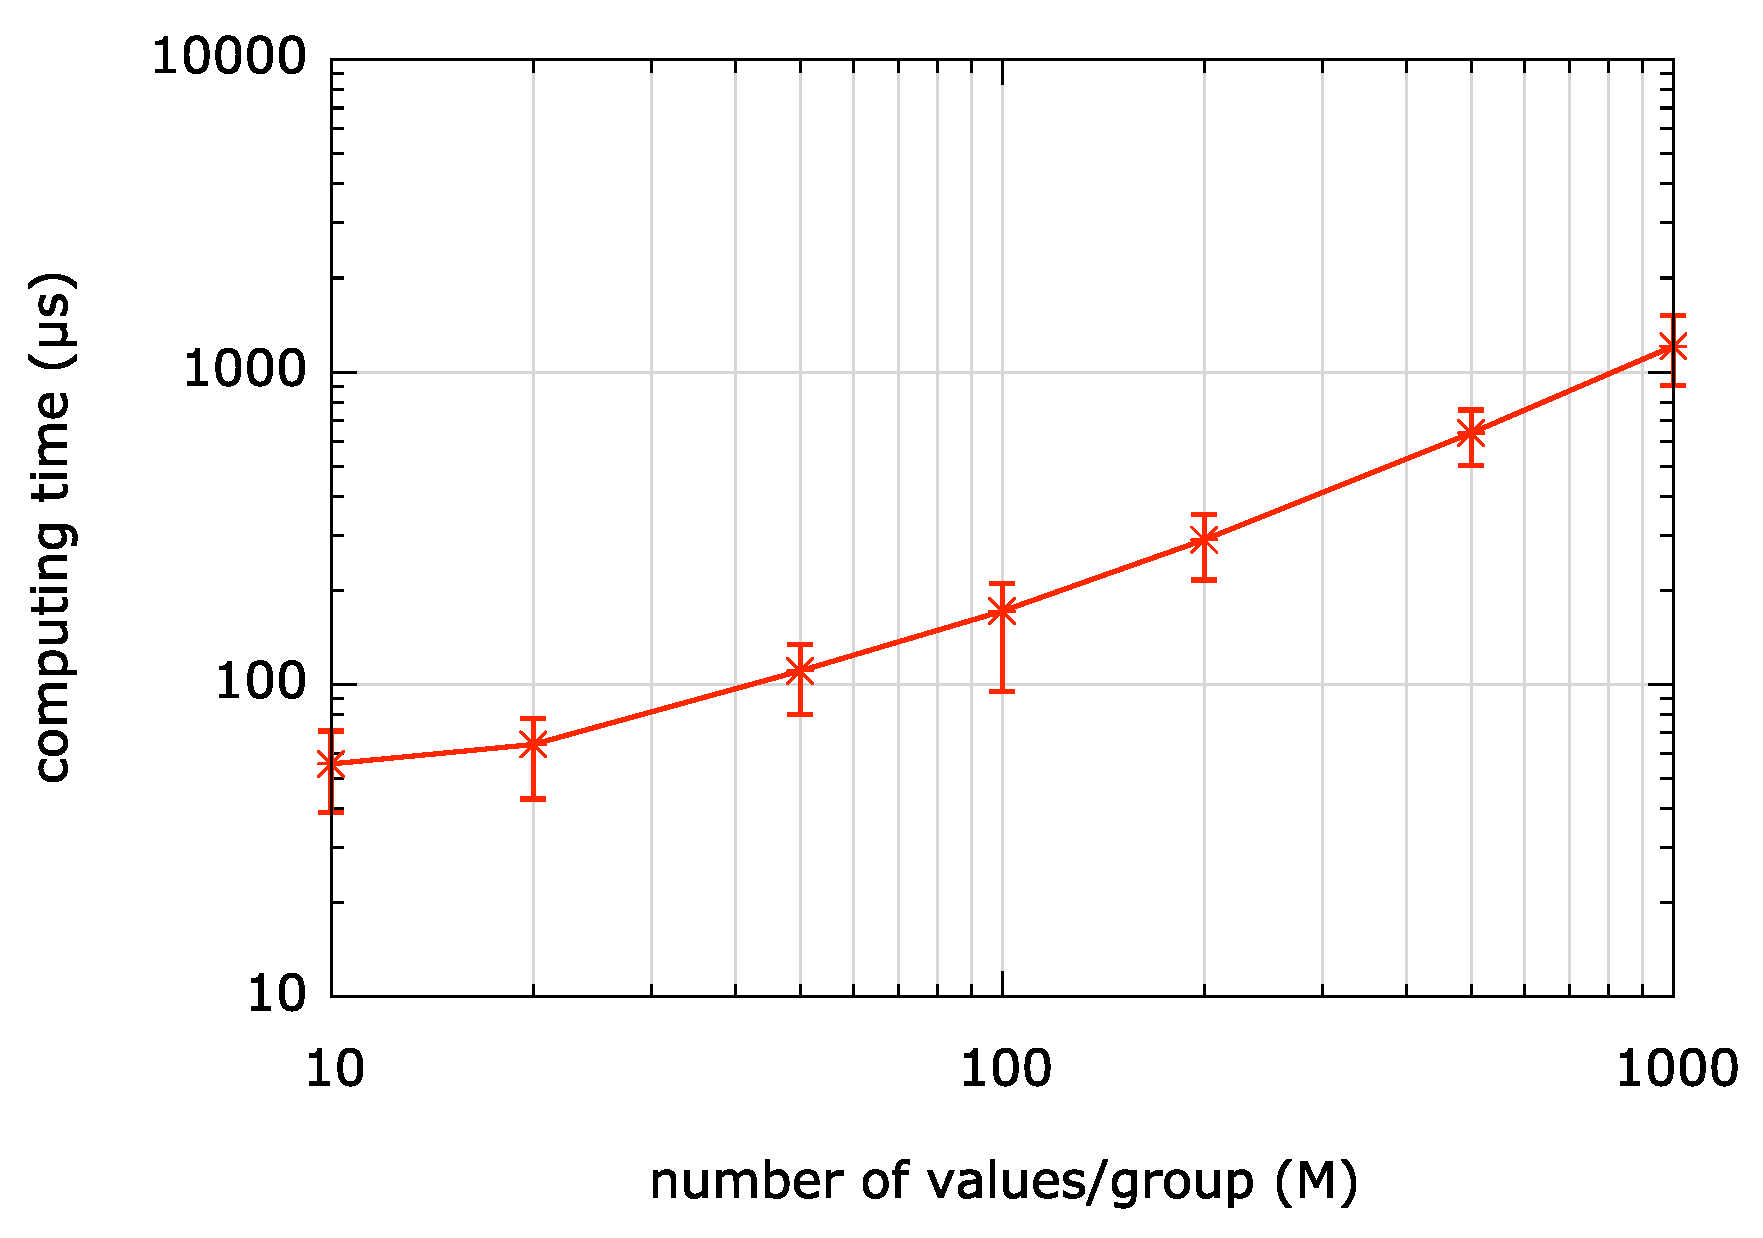
\includegraphics[width=0.48\linewidth]{valid-perfs-asteroid-aggregate-select}\label{fig:valid:perfs:asteroid:aggregate:select}}
\caption{Performance de la jointure avec agrégat en utilisant la sélection ou non}\label{fig:valid:perfs:asteroid:agg}
\end{figure}

\textbf{Résultats} : Dans cette expérience, nous avons pu remarquer que les performances de la requête \textit{SQL} de \textit{dbsource} ne dépend que de la taille de l'historique $(M.D)$. Toutefois, ce n'est pas le cas pour un agrégat utilisant une sélection sur l'identifiant avec \textit{dbjoin}, qui ne dépend principalement que de $M$. La figure~\ref{fig:valid:perfs:asteroid:aggregate} représente l'évolution de la latence de la requête d'agrégat avec et sans la sélection\footnote{La perte de performance massive observée après $4M$ de n-uplets est due au \textit{buffering} qui ne peut être fait en mémoire et le disque est utilisé. Ce fait a été confirmé par les développeurs d'\textit{H2}.}. La figure~\ref{fig:valid:perfs:asteroid:aggregate:select} représente l'évolution de la latence en variant $M$ pour l'agrégat avec sélection.

La performance dépend des caractéristiques de l'historique. Plus nous avons un $M$ petit, plus nous avons une petite latence pour le plan \textbf{P2}. La latence de \textbf{P2} est bornée entre les deux courbes de la figure~\ref{fig:valid:perfs:asteroid:aggregate} comme le cas $M=10$ représente le minimum de latence et $D=1$ (équivalent à aucune sélection) est le pire cas. Le choix du plan est clairement en faveur du plan \textbf{P2} car son pire cas a des performances similaires à \textbf{P1}. Dans l'expérience précédente, nous avions supposé pouvoir absorbé le coût de mise à jour. Ce n'est pas le cas ici car l'historique est régulièrement mis à jour.

\subsubsection{D'autres stratégies}
Si le résultat de la requête peut être dégradé, il est possible d'utiliser \textit{dbsource} est mode périodique. Dans ce cas, nous pouvons évaluer la condition limite pour passer d'un plan à l'autre en regardant les coûts mesurés dans la figure~\ref{fig:valid:perfs:asteroid:agg}.

Nous pouvons toutefois trouver une autre réécriture exacte. Lorsque la requête est déployé, il est possible de faire une distinction entre le passé $(CPUMemHistory^{t_0})$ et le futur représenté par le flux $CPUMem$. En supposant que l'agrégat est séparable par les moyens décrit dans la section~\ref{sec:rw:sgfd:optim:fenetres}, alors nous pouvons séparer les calculs sur le passé et le futur. L'agrégat passé est un calcul instantané effectué par \textit{dbsource} est mode \textit{one-shot}. L'agrégat futur est calculé par les opérateurs $_{id}\G[\infty]$. Or, ces opérateurs peuvent être regroupés en un seul macro-bloc capable de calculer l'agrégat avec un coût mémoire borné.
\section{Conclusion}
Ce chapitre a dressé un état de l'art des différents systèmes capables d'offrir une solution générique de supervision. Il en ressort qu'aucun système ne supporte entièrement les critères de qualité que nous nous sommes fixés. Le tableau~\ref{tab:rw:supervision:bilan} résume les 11 points d'analyse en colorant les différentes points suivant leurs conformités. 

\begin{sidewaystable}[ht]
\centering
\begin{tabular}{@{{\vrule width 1pt}\ \ }>{\raggedleft}m{3cm}@{\ \ {\vrule width 1pt}\ \ }M{4.2cm}|M{4.2cm}|M{4.2cm}|M{4.2cm}@{\ \ {\vrule width 1pt}}} \bottomrule
\head Critère & \head Système d'administration & \head Gestion de contexte & \head Entrepôts de données & \head Gestion de flux de données \\  \toprule \bottomrule
\critereAA & Hiérarchique & Triplets & Relationnel & Relationnel dérivé \\ \hline
\critereAB & \meh Structure hiérarchique sans contraintes & \good Ontologies & \good Modèle relationnel normalisé & \bad Pas de structure \\ \hline
\critereAC & \meh Notifications & \bad Ajout du temps en propriété & \meh CDC & \good Flux natif \\ \toprule \bottomrule
\critereBA & \meh Instantanée, continu en ad-hoc & \bad Instantané principalement & \meh Instantané. ETL en pseudo-continu & \bad Continu uniquement \\ \hline
\critereBB & \good Standardisation, union de modèles & \meh Fusion d'ontologies non standardes & \good Processus ETL (complexe) & \good Union et jointures de flux \\ \hline
\critereBC & \bad Impératif principalement & \good Logique & \meh Déclaratif (SQL) et Procédural (ETL) & \good Déclaratif principalement\\ \hline
\critereBD & \meh Procédures à écrire soi-même & \good Logique du premier ordre & \good Relationnel multidimensionnel et Algorithmie dédiée & \meh Relationnel avec support du dynamisme\\ \toprule \bottomrule
\critereCA & \good Support des standards & \meh Spécification longue des domaines & \bad Spécification du schéma, des ETL, autre (complexe) & \good Écriture de requêtes \\ \hline
\critereCB & \bad Aucune & \good Séparation par les domaines & \good Données multidimensionnelles & \bad Aucune \\ \hline
\critereCC & \good Modèle extensible, fonctions métiers dans le gestionnaire & \meh Capteurs virtuels & \good Opérateurs ETL, procédures SQL, algorithmes & \meh Sources et puits mais pas les opérateurs  \\ \hline
\critereCD & \good Large échelle & \bad Complexité très haute & \meh Réactivité lente, Support de grande quantité & \good Support de haut débits\\ \toprule 
\end{tabular}
\caption{Récapitulatif de l'état de l'art des systèmes génériques de supervision}\label{tab:rw:supervision:bilan}
\end{sidewaystable}
Il en ressort que les systèmes d'administrations sont avant tout des systèmes qui fonctionnent grâce au support des standards et à leur simplicité d'implémentation. L'architecture avec gestionnaire adaptable grâce à des langages impératifs permets une grande flexibilité pour s'adapter aux cas d'usages. De son côté, l'informatique contextuelle fournit des outils permettant de modéliser et manipuler proprement les concepts du système grâce aux ontologies et aux raisonnements logiques. Il en sort une claire séparation des domaines de compétences. Les entrepôts de données quant à eux se distinguent par des capacités d'analyses très poussées, ainsi qu'un procédé d'intégration, très complexe et lourd malheureusement, mais très complet. Enfin, la gestion de flux de données est une base solide pour gérer les données dynamiques. L'intégration et l'adaptation au système étant fait entièrement de manière déclarative en fait une solution performante et viable.

À la vue de l'état de l'art, voici les points qui vont être critique sur notre établissement de notre contribution :
\begin{itemize}
    \item La gestion de flux est un bon socle pour gérer les données dynamique grâce aux requêtes continues.
    \item Elle ne suffit pas pour constituer un système d'observation complet, notamment à l'absence de modèle de description et de requêtes instantanées.
    \item Les entrepôts et bases de données sont capables de répondre aux requêtes instantanées.
    \item Les ETL sont trop complexes à manipuler pour intégrer les données, alors que les SGFD sont plus déclaratifs.
\end{itemize}
Il devient clair que les systèmes de gestions de flux de données forment un bon candidat comme fondation pour un architecture d'observation de système. Il nous faut donc approfondir l'état de l'art technique sur ce domaine pour modeler notre contribution. Le point majeur sera d'apporter les capacités des systèmes de gestions de données relationnels. En effet, en apportant le support persistant à la gestion de flux de données, en clarifiant et augmentant son langage, nous aurons un outil qui sera plus apte à répondre à notre problématique. Ainsi, l'héritage du relationnel permettra une structure sémantique correcte, ainsi que des capacités d'analyses plus évoluées. Enfin et surtout, les données serait intégrés malgré leur hétérogénéité profonde. Le chapitre suivant détaille l'état de l'art technique de la gestion de flux de données afin de pouvoir effectuer ces améliorations.
